\chapter{Physics of Z Transverse Momentum}
\label{chapter:theory}

\section{The Standard Model}
\label{section:standard_model}

\begin{figure}[tb]
    \centering
    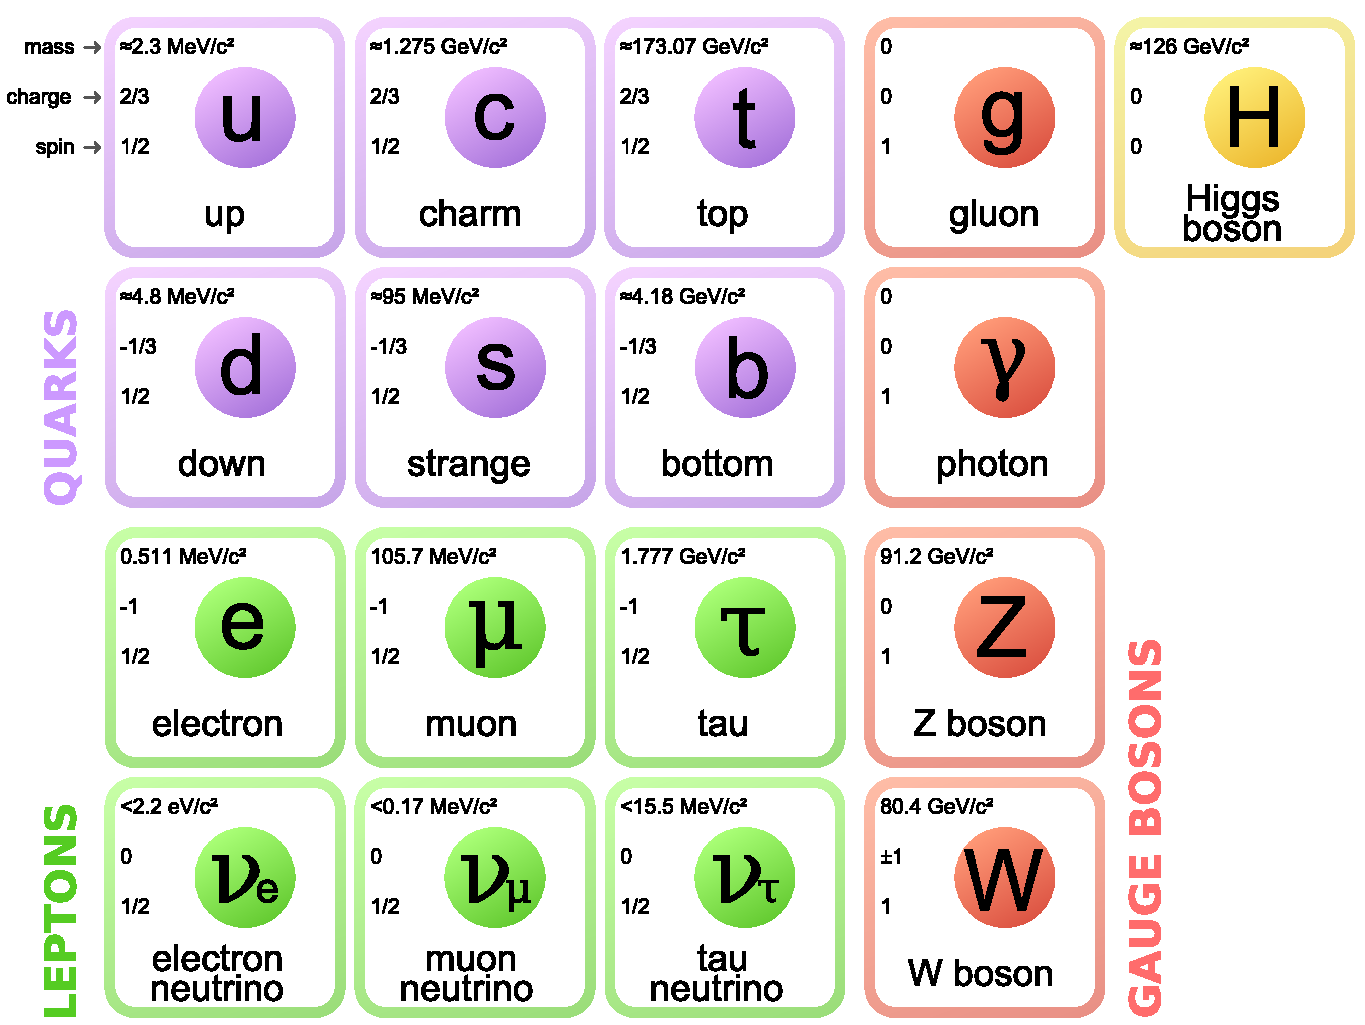
\includegraphics[width=\textwidth]{figures/standard_model.pdf}
    \caption{The particles of the standard model with information about their
        type, their mass, charge, and spin. The quarks (purple) and leptons (green)
        make up matter, while the gauge bosons (red) mediate interactions. The Higgs
        (yellow) gives mass to the Z and W bosons.
        % https://en.wikipedia.org/wiki/Standard_Model#mediaviewer/File:Standard_Model_of_Elementary_Particles.svg
        % \TODO{Source}
    }

    \label{fig:standard_model}
\end{figure}

Our current understanding of how matter interacts at high energy is entirely
described by the standard model (SM) as constructed by Weinberg, Glashow, and
Salam \cite{glashow1961}\cite{weinberg1967}\cite{salam1968}. The model combines
three of the four fundamental forces (leaving out only gravity, which is so
weak as to be negligible) and explains almost everything we see in the
universe.

\subsection{The Electromagnetic Force}
\label{subsection:electronmagnetic_force}

The modern theory of electromagnetism began with Maxwell's theory developed in
the middle of the 19th century \cite{maxwell1863}. Maxwell was the first to
conclude that light was an electromagnetic wave, the full importance of which
was only later understood when it was discovered that the photon was the force
carrier of the electromagnetic force \cite{maxwell1864}.

In the early 20th century, Lorentz and Einstein developed relativistic
mechanics and showed that Maxwell's theory was Lorentz invariant
\cite{lorentz1899}\cite{einstein1904}. Dirac updated the theory in 1920 when he
was able to quantize the electromagnetic field as an ensemble of harmonic
oscillators \cite{dirac1927}. Dirac would go on to discover that anti-particles
were a natural consequences of his equations \cite{dirac1928}\cite{dirac1930}.
These anti-particles were found by Anderson in 1932 as he observed cosmic rays
in a cloud chamber \cite{anderson1933}.

As microwave technology improved in the 1940s, more accurate measurements of
the energy level shifts in hydrogen were made, resulting in the discovery of
the Lamb shift by Lamb and Rutherford \cite{lamb1947}. This discovery pointed
to discrepancies in the theory, discrepancies which Bethe would explain after
completing a set of non-relativistic calculations using it \cite{bethe1947}.
Bethe's work inspired multiple other physicist including Dyson, Feynman,
Schwinger, and Tomonaga to work along similar lines. They created quantum
electrodynamics, a fully relativistic and self-consistent theory of
electromagnetic interactions
\cite{tomonaga1946}\cite{schwinger1948}\cite{feynman1949}\cite{dyson1949}.

\subsection{The Weak Force}
\label{subsection:weak_force}

The need for a weak force, and hence a theory describing it, was first hinted
at by beta decay experiments in the early 1900s. These experiments culminated,
in 1914, in Chadwick's discovery that the energy spectrum of electrons ejected
in beta decay was continuous instead of a delta function as would be expected
for a two-body decay \cite{chadwick1914}. While some proposed that this
discovery indicated that momentum and energy were not conserved, Pauli proposed
an alternative: there was a neutral and invisible particle that carried away
some of the energy---the neutrino \cite{pauli1930}. Fermi began working on this
idea and invented a four fermion contact interaction in which a neutron decayed
into a proton, an electron, and a neutrino \cite{fermi1934}.

In 1947, Rochester and Butler discovered a particle that decayed to two pions
which they called the $\theta$; in 1949, Brown and Powell discovered a particle
that decayed to three pions which they called the $\tau$
\cite{Rochester1947}\cite{brown1949}. It was soon discovered that these
particles had the same mass and lifetime---indicating that they were the same
particle---but, based on their decay products, they must have different parity.
Lee and Yang proposed that perhaps there was only one particle undergoing a  a
parity violating decay \cite{lee1956}. Their idea was confirmed by Wu in 1956, who
showed that electrons were preferential emitted from \cobaltsixty in one
direction, and by Garwin, Lederman, and Weinrich in 1957, who studied \pitomunu
in a storage ring \cite{wu1956}\cite{garwin1957}.

In 1954, Yang and Mills replaced Fermi's contact interaction with a non-Abelian
gauge theory that contained a spin-1 boson to mediate the force
\cite{yang1954}. However, this boson was massless, and so the weak force's
range would have been invite. In 1960, Glashow was able to modify Yang and
Mill's theory by adding Sudarshan and Marshak's vector minus axial ($V-A$)
model to produce a unified electroweak force described by the \SUtwoUone gauge
group \cite{glashow1961}\cite{sudarshan1958}. \SUtwo is a left-handed
interaction and so violates parity as expected. Weinberg and Salamn finished up
the model in 1967 when they added the Brout, Englert, and Higgs mechanism which
made the vector bosons mass and so explained the short ranged nature of the
weak interaction
\cite{weinberg1967}\cite{salam1968}\cite{englert1964}\cite{higgs1964}.

\subsection{The Strong Force}
\label{subsection:Strong_force}

The theory of the strong force grew out of studies of atomic nuclei. In 1911,
Rutherford discovered that that atomic nucleus was a compact, positively
charged object \cite{rutherford1911}. 1917, Rutherford showed that larger
nuclei were composed of hydrogen nuclei and so discovered the proton
\cite{rutherford1919}. The discovery of the uncharged neutron in 1932 by
Chadwick indicated that the atomic nucleus was made up of multiple types of
nucleons, and that it could not be held together by the electromagnetic force
\cite{chadwick1932}. In 1934, Yukawa---having noted that Fermi's contact
interaction was too weak to hold nuclei together---tried to explain this
nuclear force using meson exchange \cite{yukawa1935}. In 1947, Lettes,
Occhialini, and Powell discovered the pion which seemed to confirm Yukawa's
theory \cite{lattes1947}.

In the 1950s and early 1960s, dozens of new mesons were discovered, indicating
the need for a new theory. Some of these new mesons seemed to have a new type
of quantum number that limited their available decays, leading them to be
called ``strange'' particles. An effort to explain these particles lead to the
Gell-Mann--Nishijima formula
\cite{nakano1953}\cite{nishijima1955}\cite{gellmann1956}. This theory lead
Gell-Mann and Ne'eman to come up with a classification scheme for mesons and
baryons based on the \SUthree which Gell-Mann named the Eightfold Way. In 1964,
Gell-Mann and Zweig realized that the Eightfold Way implied that mesons were
composed of sub-atomic particles which became known as quarks
\cite{gellmann1964}\cite{zweig1964}. This model was used to predict the
existence of the charm quark, and upon its success was incorporated with
electroweak theory to form the full \SUthreeSUtwoUone symmetry group of the
standard model.

\subsection{Experimental Verification}

The standard model has been ex
